% Optics, numerical aperture, focal plan, leses, grating/filtering, detection path components, CCD, pixel array, resolution, spatial and spectroscopy resolution (nm and ev)

\subsubsection{Spectrometer}

In order to analyze different wavelengths, they need to be separated, and detected individually. This is done in a spectrometer. By shining light on a diffraction grating, the light is reflected at different angles by

\begin{equation}
d\sin(\theta _m)=m\lambda
\label{eq:grating_equation}
\end{equation}

where $d$ is the distance between the grating lines, $\theta _m$ is the outgoing angel of the light, $m$ is an integer denoting the diffraction order, and $\lambda$ is the wavelength. For large wavelength resolution, the angle of the reflected light will be large as well. So, in order to measure a large specter of wavelengths, several measurements with different center wavelengths is needed. This is due to physical limitations regarding the photo detector. There is a limit to how small a single pixel can be, and how long the array of pixels you can fit in the system. Each pixel translate to a separate wavelength, which measure the intensity of that wavelength only, which result in a full spectra of wavelengths and intensities. 

\subsubsection{Optics}

For silicon luminescence, the interesting wavelengths is from 900 to 1600nm, which corresponds to 1.38~eV and 0.77~eV (see table \ref{energy_bands}). To collect this light, the optics should have minimum loss for these wavelengths.

A common way to measure photoluminescence is to send the laser excitation light through a beam splitter, which reflects 50\% of the laser light on to the sample. Then the luminescence pass through the same beamsplitter, where 50\% is trasmitted, and into the spectrometer. For micro-photoluminescence, it's desireable to hit a very small area of the sample (order of 1~$�$m). This can be achieved by using an objective. The objective focuses the excitation laser beam with a size given by the objective spesifications in the focal plane, which is the plane of focus for the objective. The length to this plane from the objective (or other optical system), is given by its numerical aperture which in turn is given by:

\begin{equation}
NA=n sin(\theta)
\label{eq:NA}
\end{equation}

where $n$ is the refractive index of the medium in which the lens is working (1.0 for air, 1.33 for pure water), and $\theta$ is the half-angle of the maximum cone of light that can enter or exit the lens.

\begin{figure}[H]
\centering
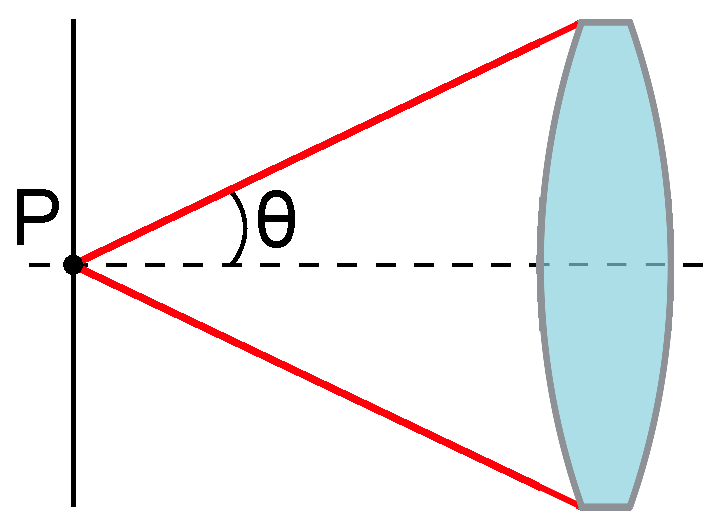
\includegraphics[width=0.5\columnwidth]{Numerical_aperture}%
\caption[Numerical aperture]{The numerical aperture with respect to a point $P$ depending on the half-angle $\theta$}%
\label{fig:NA}%
\end{figure}

where the point $P$ is the focus point. NA is important since it indicates the resolving power of a lens. The size of the details that can be resolved is proportional to $\lambda/NA$, where $\lambda$ is the wavelength of the light. A lens with a larger numerical aperture will be able to visualize finer details than a lens with a smaller numerical aperture. Lenses with larger numerical apertures also collect more light which is essential to detect luminescence of lower intensities. 

\subsubsection{Noise}

In addition to the actual photoluminescence signal, there will be noise. Noise can be from stray light in the surrounding environment hitting the camera, or it can noise from the electronics in the camera itself. Examples of noise are thermal noise, dark current, uneven amplification for different pixels in the detector, second (or more) order diffracted light from other wavelengths, background noise and different intensities for different photon energies. All measurements will be subject to noise. By having a longer integration time the signal to noise ratio is likely to increase. But a long integration time, result it a higher dark current signal. Dark current is thermally generated in the detector of the camera, and is independent of the incoming light. By cooling down the detector, the dark current noise is reduced to a minimum. This in turn makes long integration time possible, without the noise floor drowning weak signals. By blocking the signal, the dark current in addition to background light can be measures, and then subtract this noise from the measurement containing the signal. Background light should be consistent in regards to wavelength, compared to dark current, and can be subtracted more accurately. As for dark current, only an averaging is possible to subtract. This remaining white noise component is not possible to remove, and is clearly visible in areas without any signal. Second order diffraction can be a problem when pumping with a laser due to high intensities. Using a 532~nm laser to pump with, can result in second order diffraction at 1064~nm, which corresponds to 1.165~eV. The laser is reflected off the sample, and needs to be blocked before entering the spectrometer. However, it is possible that some light may slip through the filter, and with 532~nm pumping wavelength, the second order diffraction energy is right next to silicon band gap which is actual signal from the photoluminescence. By using a different pumping wavelength, or having a close to perfect filter would solve this problem.